% Schema bloc simplifie : encodeur convolutif et decodeur de type U-Net
% Usage: % Schema bloc simplifie : encodeur convolutif et decodeur de type U-Net
% Usage: % Schema bloc simplifie : encodeur convolutif et decodeur de type U-Net
% Usage: % Schema bloc simplifie : encodeur convolutif et decodeur de type U-Net
% Usage: \input{schema_bloc_autoencodeur_unet.tex}
% Preambule requis:
%   \usepackage{graphicx}
%   \usepackage{tikz}
%   \usetikzlibrary{arrows.meta, positioning, calc, decorations.pathreplacing}

\begin{tikzpicture}[
    font=\sffamily\small,
    feature/.style={draw, thick, fill=cyan!25},
    decoder/.style={draw, thick, fill=green!18},
    latent/.style={draw, thick, fill=cyan!45},
    guide/.style={densely dashed, gray, thick},
    skip/.style={densely dashed, gray, thick},
    arr/.style={-{Stealth[length=2.2mm]}, thick},
    label/.style={font=\sffamily\footnotesize, align=center}
]

% Entree et sortie
\node[draw, thick, inner sep=0pt] (input) at (0,0)
    {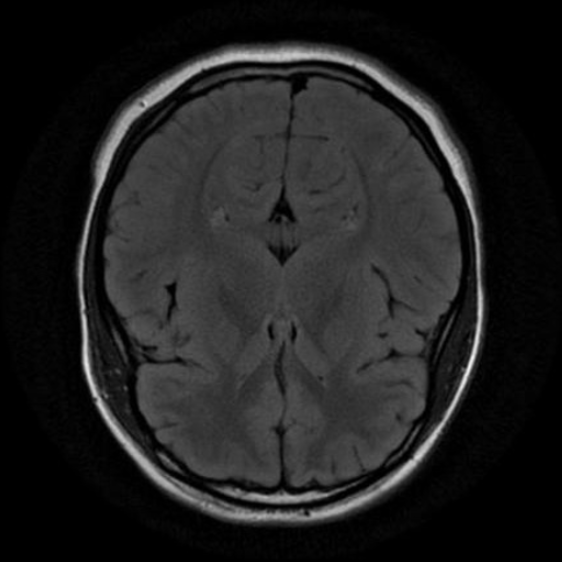
\includegraphics[width=17mm,height=17mm]{schema_bloc_unet_input_mri.png}};
\node[draw, thick, inner sep=0pt] (output) at (13.2,0)
    {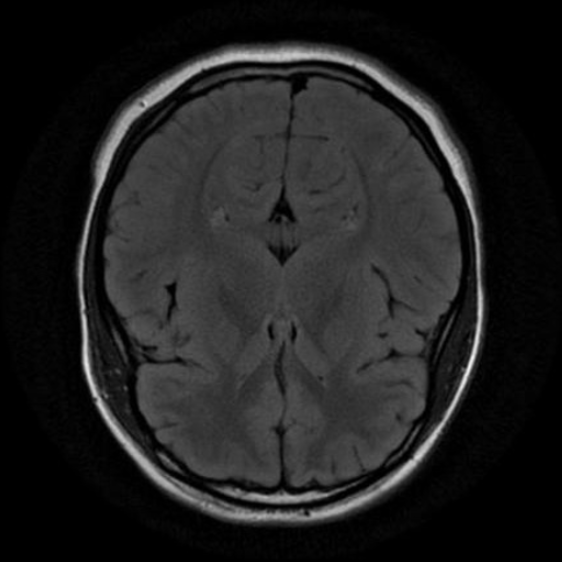
\includegraphics[width=17mm,height=17mm]{schema_bloc_unet_input_mri.png}};

% Encodeur
\node[feature, minimum width=4mm, minimum height=25mm] (e1) at (2.0,0) {};
\node[feature, minimum width=4mm, minimum height=19mm] (e2) at (3.2,0) {};
\node[feature, minimum width=4mm, minimum height=14mm] (e3) at (4.4,0) {};
\node[feature, minimum width=4mm, minimum height=9mm]  (e4) at (5.6,0) {};
\node[latent, minimum width=6mm, minimum height=6mm] (z) at (6.8,0) {$z$};

% Decodeur U-Net
\node[decoder, minimum width=4mm, minimum height=9mm]  (d1) at (8.0,0) {};
\node[decoder, minimum width=4mm, minimum height=14mm] (d2) at (9.2,0) {};
\node[decoder, minimum width=4mm, minimum height=19mm] (d3) at (10.4,0) {};
\node[decoder, minimum width=4mm, minimum height=25mm] (d4) at (11.6,0) {};

% Flux principal
\draw[arr] (input) -- (e1);
\draw[arr] (e4) -- (z);
\draw[arr] (z) -- (d1);
\draw[arr] (d4) -- (output);

% Guides visuels contraction / expansion
\foreach \a/\b in {input/e1,e1/e2,e2/e3,e3/e4,e4/z,z/d1,d1/d2,d2/d3,d3/d4,d4/output} {
    \draw[guide] (\a.north east) -- (\b.north west);
    \draw[guide] (\a.south east) -- (\b.south west);
}

% Connexions de saut U-Net
\draw[skip] (e1.north east) .. controls +(1.2,1.2) and +(-1.2,1.2) .. (d4.north west);
\draw[skip] (e2.north east) .. controls +(1.0,1.0) and +(-1.0,1.0) .. (d3.north west);
\draw[skip] (e3.north east) .. controls +(0.8,0.8) and +(-0.8,0.8) .. (d2.north west);
\node[label, above=11mm of d2] {connexions de saut};

% Labels
\node[label, below=7mm of input] {Image\\d'entree};
\node[label, below=7mm of e1] {Conv2d\\$s=2$};
\node[label, below=7mm of e2] {Conv2d\\$s=4$};
\node[label, below=7mm of e3] {$\cdots$};
\node[label, below=7mm of e4] {Conv2d\\$s=4$};
\node[label, below=7mm of z] {Vecteur\\latent};
\node[label, below=7mm of d1] {U-Net};
\node[label, below=7mm of d2] {Up};
\node[label, below=7mm of d3] {$\cdots$};
\node[label, below=7mm of d4] {Up};
\node[label, below=7mm of output] {Image\\reconstruite};

\draw[decorate, decoration={brace, mirror, amplitude=4pt}]
    ($(e1.south west)+(0,-11mm)$) -- ($(z.south east)+(0,-11mm)$)
    node[midway, below=5pt, label] {Encodeur};
\draw[decorate, decoration={brace, mirror, amplitude=4pt}]
    ($(d1.south west)+(0,-11mm)$) -- ($(d4.south east)+(0,-11mm)$)
    node[midway, below=5pt, label] {Decodeur U-Net};

\end{tikzpicture}

% Preambule requis:
%   \usepackage{graphicx}
%   \usepackage{tikz}
%   \usetikzlibrary{arrows.meta, positioning, calc, decorations.pathreplacing}

\begin{tikzpicture}[
    font=\sffamily\small,
    feature/.style={draw, thick, fill=cyan!25},
    decoder/.style={draw, thick, fill=green!18},
    latent/.style={draw, thick, fill=cyan!45},
    guide/.style={densely dashed, gray, thick},
    skip/.style={densely dashed, gray, thick},
    arr/.style={-{Stealth[length=2.2mm]}, thick},
    label/.style={font=\sffamily\footnotesize, align=center}
]

% Entree et sortie
\node[draw, thick, inner sep=0pt] (input) at (0,0)
    {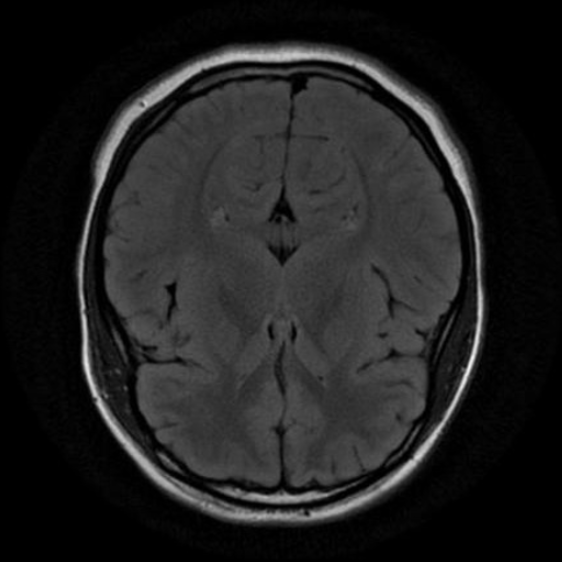
\includegraphics[width=17mm,height=17mm]{schema_bloc_unet_input_mri.png}};
\node[draw, thick, inner sep=0pt] (output) at (13.2,0)
    {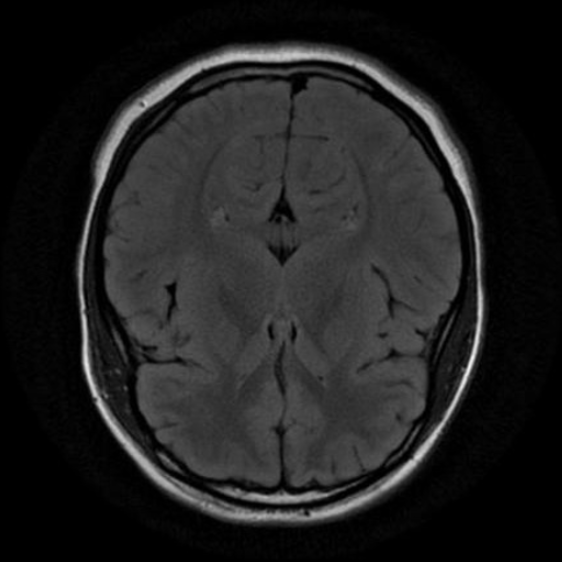
\includegraphics[width=17mm,height=17mm]{schema_bloc_unet_input_mri.png}};

% Encodeur
\node[feature, minimum width=4mm, minimum height=25mm] (e1) at (2.0,0) {};
\node[feature, minimum width=4mm, minimum height=19mm] (e2) at (3.2,0) {};
\node[feature, minimum width=4mm, minimum height=14mm] (e3) at (4.4,0) {};
\node[feature, minimum width=4mm, minimum height=9mm]  (e4) at (5.6,0) {};
\node[latent, minimum width=6mm, minimum height=6mm] (z) at (6.8,0) {$z$};

% Decodeur U-Net
\node[decoder, minimum width=4mm, minimum height=9mm]  (d1) at (8.0,0) {};
\node[decoder, minimum width=4mm, minimum height=14mm] (d2) at (9.2,0) {};
\node[decoder, minimum width=4mm, minimum height=19mm] (d3) at (10.4,0) {};
\node[decoder, minimum width=4mm, minimum height=25mm] (d4) at (11.6,0) {};

% Flux principal
\draw[arr] (input) -- (e1);
\draw[arr] (e4) -- (z);
\draw[arr] (z) -- (d1);
\draw[arr] (d4) -- (output);

% Guides visuels contraction / expansion
\foreach \a/\b in {input/e1,e1/e2,e2/e3,e3/e4,e4/z,z/d1,d1/d2,d2/d3,d3/d4,d4/output} {
    \draw[guide] (\a.north east) -- (\b.north west);
    \draw[guide] (\a.south east) -- (\b.south west);
}

% Connexions de saut U-Net
\draw[skip] (e1.north east) .. controls +(1.2,1.2) and +(-1.2,1.2) .. (d4.north west);
\draw[skip] (e2.north east) .. controls +(1.0,1.0) and +(-1.0,1.0) .. (d3.north west);
\draw[skip] (e3.north east) .. controls +(0.8,0.8) and +(-0.8,0.8) .. (d2.north west);
\node[label, above=11mm of d2] {connexions de saut};

% Labels
\node[label, below=7mm of input] {Image\\d'entree};
\node[label, below=7mm of e1] {Conv2d\\$s=2$};
\node[label, below=7mm of e2] {Conv2d\\$s=4$};
\node[label, below=7mm of e3] {$\cdots$};
\node[label, below=7mm of e4] {Conv2d\\$s=4$};
\node[label, below=7mm of z] {Vecteur\\latent};
\node[label, below=7mm of d1] {U-Net};
\node[label, below=7mm of d2] {Up};
\node[label, below=7mm of d3] {$\cdots$};
\node[label, below=7mm of d4] {Up};
\node[label, below=7mm of output] {Image\\reconstruite};

\draw[decorate, decoration={brace, mirror, amplitude=4pt}]
    ($(e1.south west)+(0,-11mm)$) -- ($(z.south east)+(0,-11mm)$)
    node[midway, below=5pt, label] {Encodeur};
\draw[decorate, decoration={brace, mirror, amplitude=4pt}]
    ($(d1.south west)+(0,-11mm)$) -- ($(d4.south east)+(0,-11mm)$)
    node[midway, below=5pt, label] {Decodeur U-Net};

\end{tikzpicture}

% Preambule requis:
%   \usepackage{graphicx}
%   \usepackage{tikz}
%   \usetikzlibrary{arrows.meta, positioning, calc, decorations.pathreplacing}

\begin{tikzpicture}[
    font=\sffamily\small,
    feature/.style={draw, thick, fill=cyan!25},
    decoder/.style={draw, thick, fill=green!18},
    latent/.style={draw, thick, fill=cyan!45},
    guide/.style={densely dashed, gray, thick},
    skip/.style={densely dashed, gray, thick},
    arr/.style={-{Stealth[length=2.2mm]}, thick},
    label/.style={font=\sffamily\footnotesize, align=center}
]

% Entree et sortie
\node[draw, thick, inner sep=0pt] (input) at (0,0)
    {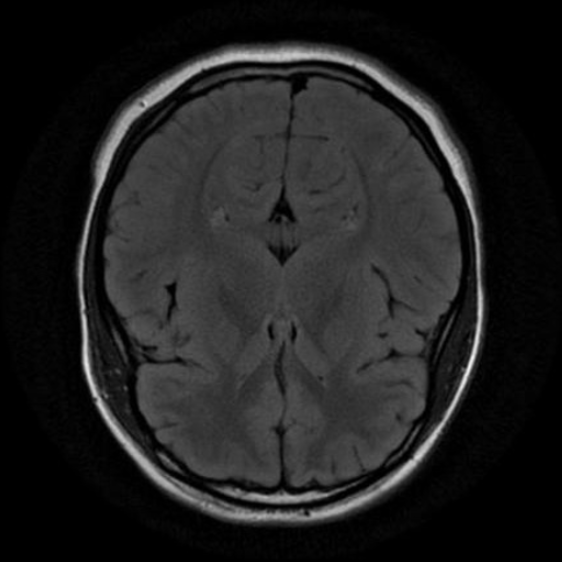
\includegraphics[width=17mm,height=17mm]{schema_bloc_unet_input_mri.png}};
\node[draw, thick, inner sep=0pt] (output) at (13.2,0)
    {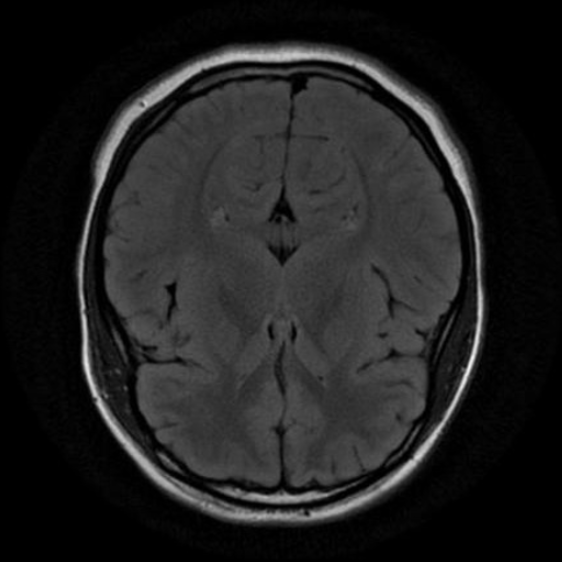
\includegraphics[width=17mm,height=17mm]{schema_bloc_unet_input_mri.png}};

% Encodeur
\node[feature, minimum width=4mm, minimum height=25mm] (e1) at (2.0,0) {};
\node[feature, minimum width=4mm, minimum height=19mm] (e2) at (3.2,0) {};
\node[feature, minimum width=4mm, minimum height=14mm] (e3) at (4.4,0) {};
\node[feature, minimum width=4mm, minimum height=9mm]  (e4) at (5.6,0) {};
\node[latent, minimum width=6mm, minimum height=6mm] (z) at (6.8,0) {$z$};

% Decodeur U-Net
\node[decoder, minimum width=4mm, minimum height=9mm]  (d1) at (8.0,0) {};
\node[decoder, minimum width=4mm, minimum height=14mm] (d2) at (9.2,0) {};
\node[decoder, minimum width=4mm, minimum height=19mm] (d3) at (10.4,0) {};
\node[decoder, minimum width=4mm, minimum height=25mm] (d4) at (11.6,0) {};

% Flux principal
\draw[arr] (input) -- (e1);
\draw[arr] (e4) -- (z);
\draw[arr] (z) -- (d1);
\draw[arr] (d4) -- (output);

% Guides visuels contraction / expansion
\foreach \a/\b in {input/e1,e1/e2,e2/e3,e3/e4,e4/z,z/d1,d1/d2,d2/d3,d3/d4,d4/output} {
    \draw[guide] (\a.north east) -- (\b.north west);
    \draw[guide] (\a.south east) -- (\b.south west);
}

% Connexions de saut U-Net
\draw[skip] (e1.north east) .. controls +(1.2,1.2) and +(-1.2,1.2) .. (d4.north west);
\draw[skip] (e2.north east) .. controls +(1.0,1.0) and +(-1.0,1.0) .. (d3.north west);
\draw[skip] (e3.north east) .. controls +(0.8,0.8) and +(-0.8,0.8) .. (d2.north west);
\node[label, above=11mm of d2] {connexions de saut};

% Labels
\node[label, below=7mm of input] {Image\\d'entree};
\node[label, below=7mm of e1] {Conv2d\\$s=2$};
\node[label, below=7mm of e2] {Conv2d\\$s=4$};
\node[label, below=7mm of e3] {$\cdots$};
\node[label, below=7mm of e4] {Conv2d\\$s=4$};
\node[label, below=7mm of z] {Vecteur\\latent};
\node[label, below=7mm of d1] {U-Net};
\node[label, below=7mm of d2] {Up};
\node[label, below=7mm of d3] {$\cdots$};
\node[label, below=7mm of d4] {Up};
\node[label, below=7mm of output] {Image\\reconstruite};

\draw[decorate, decoration={brace, mirror, amplitude=4pt}]
    ($(e1.south west)+(0,-11mm)$) -- ($(z.south east)+(0,-11mm)$)
    node[midway, below=5pt, label] {Encodeur};
\draw[decorate, decoration={brace, mirror, amplitude=4pt}]
    ($(d1.south west)+(0,-11mm)$) -- ($(d4.south east)+(0,-11mm)$)
    node[midway, below=5pt, label] {Decodeur U-Net};

\end{tikzpicture}

% Preambule requis:
%   \usepackage{graphicx}
%   \usepackage{tikz}
%   \usetikzlibrary{arrows.meta, positioning, calc, decorations.pathreplacing}

\begin{tikzpicture}[
    font=\sffamily\small,
    feature/.style={draw, thick, fill=cyan!25},
    decoder/.style={draw, thick, fill=green!18},
    latent/.style={draw, thick, fill=cyan!45},
    guide/.style={densely dashed, gray, thick},
    skip/.style={densely dashed, gray, thick},
    arr/.style={-{Stealth[length=2.2mm]}, thick},
    label/.style={font=\sffamily\footnotesize, align=center}
]

% Entree et sortie
\node[draw, thick, inner sep=0pt] (input) at (0,0)
    {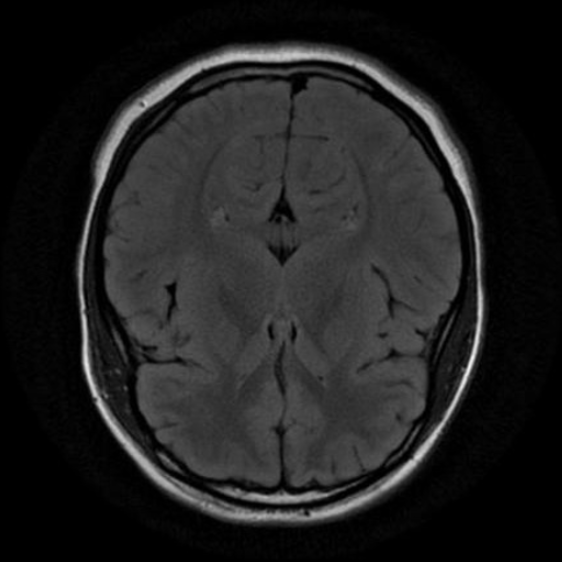
\includegraphics[width=17mm,height=17mm]{schema_bloc_unet_input_mri.png}};
\node[draw, thick, inner sep=0pt] (output) at (13.2,0)
    {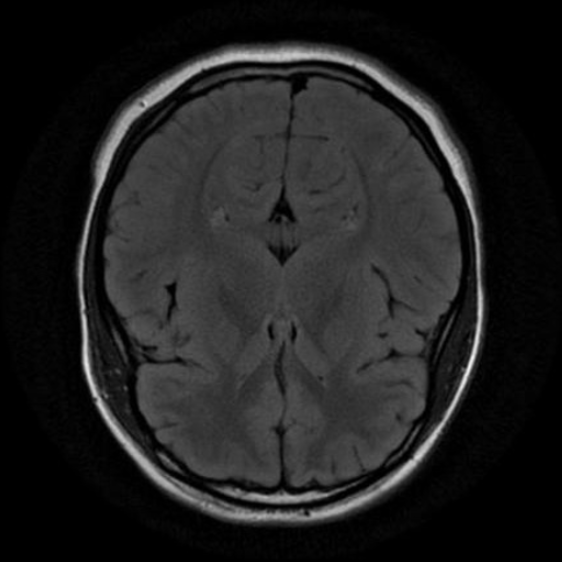
\includegraphics[width=17mm,height=17mm]{schema_bloc_unet_input_mri.png}};

% Encodeur
\node[feature, minimum width=4mm, minimum height=25mm] (e1) at (2.0,0) {};
\node[feature, minimum width=4mm, minimum height=19mm] (e2) at (3.2,0) {};
\node[feature, minimum width=4mm, minimum height=14mm] (e3) at (4.4,0) {};
\node[feature, minimum width=4mm, minimum height=9mm]  (e4) at (5.6,0) {};
\node[latent, minimum width=6mm, minimum height=6mm] (z) at (6.8,0) {$z$};

% Decodeur U-Net
\node[decoder, minimum width=4mm, minimum height=9mm]  (d1) at (8.0,0) {};
\node[decoder, minimum width=4mm, minimum height=14mm] (d2) at (9.2,0) {};
\node[decoder, minimum width=4mm, minimum height=19mm] (d3) at (10.4,0) {};
\node[decoder, minimum width=4mm, minimum height=25mm] (d4) at (11.6,0) {};

% Flux principal
\draw[arr] (input) -- (e1);
\draw[arr] (e4) -- (z);
\draw[arr] (z) -- (d1);
\draw[arr] (d4) -- (output);

% Guides visuels contraction / expansion
\foreach \a/\b in {input/e1,e1/e2,e2/e3,e3/e4,e4/z,z/d1,d1/d2,d2/d3,d3/d4,d4/output} {
    \draw[guide] (\a.north east) -- (\b.north west);
    \draw[guide] (\a.south east) -- (\b.south west);
}

% Connexions de saut U-Net
\draw[skip] (e1.north east) .. controls +(1.2,1.2) and +(-1.2,1.2) .. (d4.north west);
\draw[skip] (e2.north east) .. controls +(1.0,1.0) and +(-1.0,1.0) .. (d3.north west);
\draw[skip] (e3.north east) .. controls +(0.8,0.8) and +(-0.8,0.8) .. (d2.north west);
\node[label, above=11mm of d2] {connexions de saut};

% Labels
\node[label, below=7mm of input] {Image\\d'entree};
\node[label, below=7mm of e1] {Conv2d\\$s=2$};
\node[label, below=7mm of e2] {Conv2d\\$s=4$};
\node[label, below=7mm of e3] {$\cdots$};
\node[label, below=7mm of e4] {Conv2d\\$s=4$};
\node[label, below=7mm of z] {Vecteur\\latent};
\node[label, below=7mm of d1] {U-Net};
\node[label, below=7mm of d2] {Up};
\node[label, below=7mm of d3] {$\cdots$};
\node[label, below=7mm of d4] {Up};
\node[label, below=7mm of output] {Image\\reconstruite};

\draw[decorate, decoration={brace, mirror, amplitude=4pt}]
    ($(e1.south west)+(0,-11mm)$) -- ($(z.south east)+(0,-11mm)$)
    node[midway, below=5pt, label] {Encodeur};
\draw[decorate, decoration={brace, mirror, amplitude=4pt}]
    ($(d1.south west)+(0,-11mm)$) -- ($(d4.south east)+(0,-11mm)$)
    node[midway, below=5pt, label] {Decodeur U-Net};

\end{tikzpicture}
